%%%%%%%%%%%%%%%%%%%%%%%%%%%%%%%%%%%%%%%%%%%%%%%%%%%%%%%%%%%%%%%%%%%%%%%%%%%%%%%%
\documentclass[twocolumn]{revtex4}

%%%%%%%%%%%%%%%%%%%%%%%%%%%%%%%%%%%%%%%%%%%%%%%%%%%%%%%%%%%%%%%%%%%%%%%%%%%%%%%%
% Note that comments begin with a "%" and are not turned into text in the .pdf
% document.
%%%%%%%%%%%%%%%%%%%%%%%%%%%%%%%%%%%%%%%%%%%%%%%%%%%%%%%%%%%%%%%%%%%%%%%%%%%%%%%%

%%%%%%%%%%%%%%%%%%%%%%%%%%%%%%%%%%%%%%%%%%%%%%%%%%%%%%%%%%%%%%%%%%%%%%%%%%%%%%%%
% Include some extra packages.
%%%%%%%%%%%%%%%%%%%%%%%%%%%%%%%%%%%%%%%%%%%%%%%%%%%%%%%%%%%%%%%%%%%%%%%%%%%%%%%%
\usepackage[]{graphicx}
\usepackage[procnames]{listings}
\usepackage{color}
%%%%%%%%%%%%%%%%%%%%%%%%%%%%%%%%%%%%%%%%%%%%%%%%%%%%%%%%%%%%%%%%%%%%%%%%%%%%%%%%

%%%%%%%%%%%%%%%%%%%%%%%%%%%%%%%%%%%%%%%%%%%%%%%%%%%%%%%%%%%%%%%%%%%%%%%%%%%%%%%%
\begin{document}
\definecolor{keywords}{RGB}{255,0,90}
\definecolor{comments}{RGB}{0,0,113}
\definecolor{red}{RGB}{160,0,0}
\definecolor{green}{RGB}{0,150,0}
% as note theese colors were used for the python code and how to insert python code I found from https://python.g-node.org/python-summerschool-2009/python_code_in_latex


%%%%%%%%%%%%%%%%%%%%%%%%%%%%%%%%%%%%%%%%%%%%%%%%%%%%%%%%%%%%%%%%%%%%%%%%%%%%%%%%
\title{
Escaping the Raptor
}

\author{A.~Maciaszek}
\affiliation{Siena College, Loudonville, NY}

\date{\today}

\begin{abstract}
    The object of this project is to find the out how this scenario of myself and raptor in a predator versus prey chase. The variables such as my speed the raptors have been given as well as from how far it can attack from, the amount of attacks it will make and chance of each their success. I have concluded that the raptor will be within attacking range with in 5.8 meters within 1.93 second and will have a 63 percent chance of survivng all three attacks the raptor makes.
    
\end{abstract}

\maketitle
%%%%%%%%%%%%%%%%%%%%%%%%%%%%%%%%%%%%%%%%%%%%%%%%%%%%%%%%%%%%%%%%%%%%%%%%%%%%%%%%

%%%%%%%%%%%%%%%%%%%%%%%%%%%%%%%%%%%%%%%%%%%%%%%%%%%%%%%%%%%%%%%%%%%%%%%%%%%%%%%%
\section{Introduction}
For this scenario the raptors speed is 18 meters per second and it accelerates to this instantly (to simplify calculations) and I will be already at running speed of 3 meters per second and both of us will be traviling at a constant rate.

First I created equations that took the time in and gave you the position for both myself running and the raptor.
$$Raptorposition= 18*t$$ $$My  position= 18*t$$
    
I then made a graph of both these functions in python
    
\begin{figure}[h]
  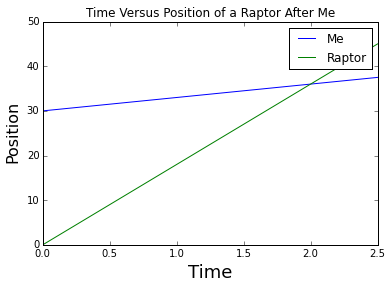
\includegraphics[width=90mm]{graph1.png}
  \caption{In this graph it shows where the raptor and myself are in relation to time}
\textit{\textit{•\textbf{•}}}  \label{fig:graph1}
\end{figure}
%%%%%%%%%%%%%%%%%%%%%%%%%%%%%%%%%%%%%%%%%%%%%%%%%%%%%%%%%%%%%%%%%%%%%%%%%%%%%%%%


%%%%%%%%%%%%%%%%%%%%%%%%%%%%%%%%%%%%%%%%%%%%%%%%%%%%%%%%%%%%%%%%%%%%%%%%%%%%%%%%
\section{Meeting the Raptor}
For this scenario the raptors speed is 18 meters per second and it accelerates to this instantly (to simplify calculations) and I will be already at running speed of 3 meters per second and both of us will be traviling at a constant rate.

First I created equations that took the time in and gave you the position for both myself running and the raptor.
$$Raptorposition= 18*t$$ $$My  position= 18*t$$
    
I then made a graph of both these functions in python
    
\begin{figure}[h]
  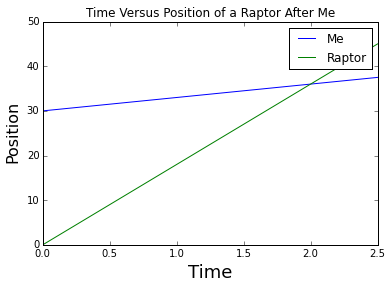
\includegraphics[width=90mm]{graph1.png}
  \caption{In this graph it shows where the raptor and myself are in relation to time}
\textit{\textit{•\textbf{•}}}  \label{fig:graph1}
\end{figure}
%%%%%%%%%%%%%%%%%%%%%%%%%%%%%%%%%%%%%%%%%%%%%%%%%%%%%%%%%%%%%%%%%%%%%%%%%%%%%%%%
\section{Attacking}
%%%%%%%%%%%%%%%%%%%%%%%%%%%%%%%%%%%%%%%%%%%%%%%%%%%%%%%%%%%%%%%%%%%%%%%%%%%%%%%%
To calculate where the raptor would meet me is by setting up a while loop with a nested conditional. This conditional which would break when the equation of the raptor was greater than that of myself if not it would add .001 seconds to the time.
\lstset{language=Python, 
        basicstyle=\ttfamily\scriptsize, 
        keywordstyle=\color{keywords},
        commentstyle=\color{comments},
        stringstyle=\color{red},
        showstringspaces=false,
        identifierstyle=\color{green},
        procnamekeys={def,class}}
\begin{lstlisting}
t=0
while t<2:
    if 18*t>=3*t+30:
        break
    else:
        t+=float(.00001)

print 'The raptor will catch up to me in %f seconds' %t

finaldist=3*t+30
initialdist=3*0+30
dist=finaldist-initialdist
print 'The distance that I run is %f meters' %dist   
\end{lstlisting}
My code returned that it would take 2 seconds for the raptor to catch up to me and I would have traveled a distance of 6 meters. To check my work I did the problem algebraically
    $$3x+30=18t$$ 
    $$30=15t$$
    $$2=t$$
    $$(3*(2)+30)-(3*(0)+30)=6$$
    

Assuming the raptor could attack me when he was within one meter I changed the the raptors equation to $=18t+1$ and then did the same process as the previous problem.
\lstset{language=Python,} 
\begin{lstlisting}
t=0
while t<2:
    if 18*t+1>=3*t+30:
        break
    else:
        t+=float(.00001)

print 'The raptor will catch up to me in %f seconds' %t

finaldist=3*t+30
initialdist=3*0+30
dist=finaldist-initialdist
print 'The distance that I run is %f meters' %dist    
\end{lstlisting}
My code returned that it would take 1.933340 seconds for the raptor to catch up to me and I would have traveled a distance of 5.800020 meters.
To check my work for this one I also calculated it using algebra
    $$3t+30=18t+1$$
    $$29=15t$$
    $$\frac{29}{15}=t=1.93$$
    $$(3*(\frac{29}{15})+30)-(3*(0)+30)=\frac{29}{5}=5.8$$

%\begin{figure}[h]
%  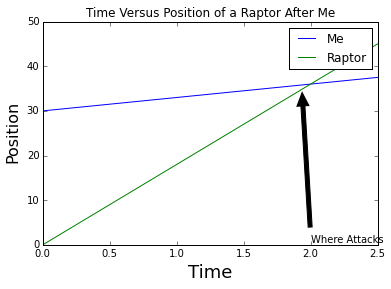
\includegraphics[width=90mm]{graph2.png}
%  \caption{In this graph it shows where the raptor is within one meter and can attack me.}
%  \label{fig:graph2}
%\end{figure}

This raptor when is close enough to attack it will attack me with a 20\% likelihood of hitting me will try again with a 15\% chance and then will try a final time with a 7\% chance.


To calculate the odds of me getting away I used a function for binary distribution set the trials equal to one and the probability to the first attacks chance of success and had it repeat this a hundred thousand times. The answer gave an array of ones which signified that person lived and zeros which meant that person died. I used another function to count the number that lived through the first attack and then used the binomial function again. This time with the different probability and instead of repeating a hundred thousand times it repeated for the amount of people who survived the first attack. I then repeated this for the third attack with those who survived the second attack. I then had the program divide the amount that survived by the original amount and then convert it to  a percent.
\begin{lstlisting}
numpe=100000000
bite1=np.random.binomial(1, .8, numpe)
live1=np.count_nonzero(bite1)
bite2=np.random.binomial(1, .85, live1)
live2=np.count_nonzero(bite2)
bite3=np.random.binomial(1, .93, live2)
live3=np.count_nonzero(bite3)
alive=(float(live3)/numpe)*100
print 'Probability I will survive attacks is %s %' %alive
\end{lstlisting}
My code would give me roughly 63.243951 percent as my chance of surviving all attacks. To check this viability I calculated the theoretical probability
$$(\frac{80}{100}*\frac{85}{100}*\frac{93}{100})*100=63.24$$
%%%%%%%%%%%%%%%%%%%%%%%%%%%%%%%%%%%%%%%%%%%%%%%%%%%%%%%%%%%%%%%%%%%%%%%%%%%%%%%%

%%%%%%%%%%%%%%%%%%%%%%%%%%%%%%%%%%%%%%%%%%%%%%%%%%%%%%%%%%%%%%%%%%%%%%%%%%%%%%%%
\end{document}
%%%%%%%%%%%%%%%%%%%%%%%%%%%%%%%%%%%%%%%%%%%%%%%%%%%%%%%%%%%%%%%%%%%%%%%%%%%%%%%%
